\appendix

\FloatBarrier
\section{Dataset laws and partitions}
\label{app:data}

\begin{figure}[htbp]
\centering
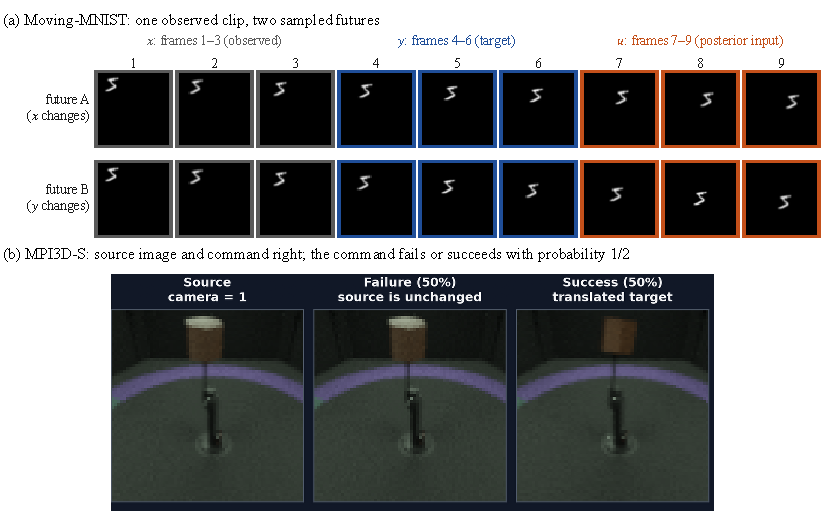
\includegraphics[width=\linewidth]{figures/dataset_protocols.pdf}
\caption{What the models observe and predict. (a) Moving-MNIST, rendered by the generator used for all runs (training identity \texttt{\VFigMMIdentity}, digit \VFigMMDigit). The source velocity is \VFigMMVelocity{} px/frame, and the two rows show two sampled futures with new velocities \VFigMMFutureA{} and \VFigMMFutureB. The example is illustrative; its seed rule is given below. (b) MPI3D-S: the stochastic-execution row of our rendering of the official archive, cropped without restyling. Source factors are colour 4, shape 3, size 1, camera 1 and position $(20,20)$, with the command right. The residue $(4+3+3\cdot1)\bmod6=4$ makes this a \emph{validation}-split object.}
\label{fig:data}
\end{figure}

\begin{table}[htbp]
\caption{Dataset construction and evaluation populations derived from the generator, the split code and the evaluation protocol.}
\label{tab:data}
\label{tab:overview}
\centering
\small
\begin{tabular}{@{}p{0.29\linewidth}p{0.66\linewidth}@{}}
\toprule
\multicolumn{2}{@{}l}{\textbf{Moving-MNIST}} \\
\midrule
Image source & MNIST, 28$\times$28 digits \\
Identity partition & 50,000 train / 10,000 development (5,000 selection, 5,000 report) / 10,000 official test \\
Training examples & fresh online clips; 75{,}000 updates $\times$ 128 = 9.6M presentations \\
Observed $x$ / target $y$ & frames 1--3 / frames 4--6 \\
Posterior input $u$ (training) & frames 7--9 of the same trajectory \\
Readout and probe fit & 8,192 clips, train identities \\
Readout and probe selection & 2,048 clips, development selection identities \\
Final report / forecast queries & 2,048 / 1,024 clips, official test identities \\
Draws per query & 64 forecast, 128 physical truth \\
\midrule
\multicolumn{2}{@{}l}{\textbf{MPI3D-S (balanced stochastic execution)}} \\
\midrule
Image source & MPI3D-realistic, 64$\times$64, background fixed \\
Attribute split & 48 / 12 / 12 colour--shape--size combinations \\
Training population & 589,824 source/command pairs (48 $\times$ 3 cameras $\times$ 1,024 positions $\times$ 4) \\
Training examples & 100 epochs $\times$ 65,536 = 6.55M presentations, 102,400 updates \\
Observed $x,a$ / target $y$ & source image and unit command / realized next image \\
Posterior input $u$ (training) & the realized target $y$ itself \\
Readout fit / select / hold-out & 8,192 / 2,048 / 2,048 train-attribute images (of 230,400) \\
Probe fit / select / report & 8,192 train / 2,048 validation / 2,048 test images \\
Forecast queries & 2,048 = 512 test sources $\times$ 4 commands (of 36,864) \\
Truth and forecast support & exact two outcomes; 16 equal-weight prior quantiles \\
\bottomrule
\end{tabular}

\end{table}

\subsection{Moving-MNIST}

\paragraph{Law and rendering.} Coordinates are $(x,y)$ in pixels, with the origin at the top-left pixel centre and $y$ increasing downward; velocities are in px/frame. For a source state with centre $c_0$ and velocity $v$,
\begin{align*}
c_0&\sim\mathcal U[8,16]^2,\quad v\sim\mathcal U[0,3]^2,\quad k\sim\mathrm{Bernoulli}(\tfrac12),\quad \epsilon\sim\mathcal N(0,1),\\
v'_k&=v_k+\tfrac23 v_k\,\epsilon,\qquad v'_{1-k}=v_{1-k},\\
c_t&=c_0+(t-1)\,v\quad(t=1,2,3),\qquad c_t=c_0+2v+(t-3)\,v'\quad(t=4,\dots,9).
\end{align*}
Here $k=1$ means that the vertical component changes. A $28{\times}28$ digit is scaled to $[0,1]$, resized to $16{\times}16$ by antialiased bilinear interpolation (\texttt{align\_corners=False}), and placed by bilinear grid sampling with zero padding. A digit centred at $c$ has its leftmost pixel centre at $c-7.5$. Frames outside the canvas are cropped. There is no bounce, and velocities are never clipped or resampled. Clips have shape $(1,3,64,64)$: $x$ is frames 1--3, $y$ frames 4--6, and $u$ frames 7--9. The Gaussian scale is read as a standard deviation. Under a variance reading the conditional variance on the changed axis would be $\tfrac23v_k$ instead of $(\tfrac23v_k)^2$, which would need a different generator (Appendix~\ref{app:fidelity}).

\paragraph{Identity manifest.} The identity manifest has content hash \texttt{fd4a5cab\ldots1784}, equal to the value recorded in the evaluation protocol fixed before main training. It permutes the official training indices with \texttt{numpy} PCG64 seed 0. The first 50{,}000 indices (stored sorted) become training identities, the remaining 10{,}000 become development identities, and all 10{,}000 official test images become test identities. Identifiers are namespaced (\texttt{mnist-train:NNNNN}, \texttt{mnist-test:NNNNN}), so indices cannot collide across the two files. Before any data access, the loader verifies the raw MNIST files against the checksums recorded in the manifest. Table~\ref{tab:mmbanks} maps these identity populations to the evaluation banks.

\begin{table}[htbp]
\caption{Moving-MNIST bank mapping. All banks are generated online from addressed random streams, with identities drawn with replacement from the listed population. Every run's readout and probes are fitted and selected on the fit and selection banks. The development report and query banks served only the development replication; the final banks produced every reported main-run score.}
\label{tab:mmbanks}
\centering
\small
\begin{tabular}{@{}p{0.19\linewidth}p{0.29\linewidth}p{0.3\linewidth}r@{}}
\toprule
Bank & Identity population & Used for & Clips \\
\midrule
Fit & 50{,}000 training identities & readout and probe fitting & 8{,}192 \\
Selection & development identities, first half (5{,}000) & readout penalty/transform; probe early stopping & 2{,}048 \\
Development report / queries & development identities, second half (5{,}000) & development replication only & 2{,}048 / 1{,}024 \\
Final report & 10{,}000 official test identities & probe and readout reporting & 2{,}048 \\
Final queries & 10{,}000 official test identities & primary physical score & 1{,}024 \\
\bottomrule
\end{tabular}
\end{table}

\paragraph{Visibility.} Truth futures are rendered for frames 4--6 of the first 64 of the 128 truth draws of each final query. None was blank (zero pixel mass). A fraction $1.73\times10^{-4}$ of them were geometrically cropped, meaning that the nominal $16{\times}16$ box left the canvas. Cropping therefore affects very few rendered targets in the final bank.

\paragraph{Illustration seed.} The example in Figure~\ref{fig:data}a uses training identity \texttt{\VFigMMIdentity}. Its seed is the first $s=0,1,\dots$ such that \texttt{SeedSequence([20260930, s])} gives both initial velocity components $\ge1.2$ px/frame, the first $x$-changed and first $y$-changed of 16 future draws each change the velocity by $\ge1$ px/frame, and all nine digit centres of both futures lie in $[9,55]$. That is $s=\VFigMMSeed$. The rule was chosen for visibility, and the example is not an evaluation query.

\subsection{MPI3D-S}

\paragraph{Factors and state.} MPI3D-realistic has seven factors: object colour (6), shape (6), size (2), camera height (3), background colour (3), and horizontal and vertical position (40 each). That makes $6\cdot6\cdot2\cdot3\cdot3\cdot40\cdot40=1{,}036{,}800$ images of $64{\times}64$ pixels. The SHA256 of the MPI3D archive used here is recorded in the evaluation protocol (\texttt{f6124f35\ldots}). We fix the background at index 0. Camera height varies across examples but never within a transition. Commands are left $(-1,0)$, right $(1,0)$, up $(0,-1)$ and down $(0,1)$ on the (horizontal, vertical) position indices. Success adds $4a$ to the position, and failure leaves the image unchanged.

\paragraph{Training sampler.} Sources are restricted to the common legal region $[4,35]^2$ (1{,}024 positions), so every command is legal and targets lie in $[0,39]^2$. Each epoch takes 65{,}536 distinct source/command pairs, without replacement, from the \VMPTrainPairs{} training pairs ($48$ attribute combinations $\times$ 3 camera heights $\times$ 1{,}024 positions $\times$ 4 commands). It assigns exactly 32{,}768 of them to failure and 32{,}768 to success, in shuffled order. This is a balanced quota, not a sequence of independent Bernoulli draws. Over 100 epochs the models see 6.55M presentations in 102{,}400 updates.

\paragraph{Split integrity.} We assign attribute combinations using $(\mathrm{colour}+\mathrm{shape}+3\,\mathrm{size})\bmod6$: residues 0--3 train, 4 validation and 5 test. Table~\ref{tab:mpsplit} lists the split counts. The three attribute sets are disjoint by construction. Position manifests are shared across splits: 64 of the 256 test positions also occur in the probe-train manifest. Images are therefore separated by attribute combination, not by position. Training transitions use all 1{,}024 legal source positions with training attributes. Readout images use training attributes at all 1{,}600 positions.

\begin{table}[htbp]
\caption{MPI3D split counts, computed from the split code and position manifests. The test position manifest's SHA256 (\texttt{75fc0370\ldots}) equals the value recorded for the final query bank.}
\label{tab:mpsplit}
\centering
\small
\begin{tabular}{@{}lrrr@{}}
\toprule
 & Train & Validation & Test \\
\midrule
Attribute combinations (residues) & 48 (0--3) & 12 (4) & 12 (5) \\
Combinations per colour / shape / size level & 8 / 8 / 24 & 2 / 2 / 6 & 2 / 2 / 6 \\
Source positions & 1{,}024 (all legal) & 128 (manifest) & 256 (manifest) \\
Source/command pairs & 589{,}824 & 18{,}432 & 36{,}864 \\
Clean probe images & 36{,}864 & 4{,}608 & 9{,}216 \\
Role in final evaluation & readout and probe fit & probe selection & queries, probe report \\
\bottomrule
\end{tabular}
\end{table}

\paragraph{Query construction.} The final query bank permutes the 9{,}216 test sources with a fixed evaluation stream, keeps the first 512, and includes all four commands for each. The two outcome images of every query are enumerated in failure-then-success order. Wrong-source controls shift sources cyclically within each evaluation batch, choosing a shift under which no query keeps its own source factors.

\paragraph{Sources and licences.} MPI3D is distributed under a Creative Commons Attribution 4.0 licence (official repository \texttt{rr-learning/disentanglement\_dataset}). MNIST was used through the official distribution files, verified by checksum; we found no licence statement on the official MNIST page.

\FloatBarrier
\section{Architecture and optimization}
\label{app:arch}

\begin{table}[htbp]
\caption{Training recipes. EMA momentum applies to the EMA models, SIGReg to the Shared models and the KL term to the variational models.}
\label{tab:training}
\centering
\small
\begin{tabular}{@{}>{\raggedright\arraybackslash}p{0.22\linewidth}>{\raggedright\arraybackslash}p{0.34\linewidth}>{\raggedright\arraybackslash}p{0.38\linewidth}@{}}
\toprule
 & Moving-MNIST & MPI3D \\
\midrule
Encoder; projector & 3D CNN, 5 layers, 768-d pooled; 768$\to$1024$\to$1024$\to$128 & ViT (patch 8, width 256, depth 6, 8 heads), mean-pooled; 256$\to$1024$\to$1024$\to$128 \\
Predictor input; residual & $z_x$ or $[z_x, r]$; $d_r{=}2$, softplus std & $[z_x, a, r]$ ($r{=}0$ for Det models); $d_r{=}1$, clamped log-std \\
Stored parameters (M), BYOL reference / AdaSSL reference / Shared-Det / Shared-Var & 6.03 / 6.44 / 3.67 / 4.08 & 10.70 / 11.11 / 6.01 / 6.42 \\
Batch; updates & 128; 75,000 & 64 (4 GPUs); 102,400 \\
AdamW learning rate & 0.0001, cosine to 0 & 0.001, 10-epoch warm-up, cosine over 1.25$\times$ budget \\
Weight decay & 0.0001, all parameters & 0.04$\to$0.4; no decay on norms and most biases (App.~\ref{app:optim}) \\
EMA momentum (EMA models) & 0.996, constant & 0.996$\to$1, cosine \\
$\beta$ (Var models); $\lambda$ (Shared models) & 0.001; 0.1 (128 directions, 17 knots, $[0.2,4]$) & same \\
\bottomrule
\end{tabular}

\end{table}

\subsection{Model details}
\label{app:modeldetails}

The EMA models update their target parameters as $\bar\theta\leftarrow\tau\bar\theta+(1-\tau)\theta$ once after every optimizer step. Only parameters are averaged; the EMA copy keeps its own BN running statistics, which its training-mode target passes update. In the Shared models every forward pass (source, target and, for \shvar{} on Moving-MNIST, the posterior clip $u$) updates the one set of BN statistics. The alignment loss is the same negative batch-mean cosine in every model, and it is not scaled by $1-\lambda$ as in LeJEPA.

The posterior of the \emavar{} consumes differentiable online features: $f(x)$ and $f(u)$ on Moving-MNIST, and $f(x)$, $a$ and an extra online encoding $f(y)$ on MPI3D. Only the EMA alignment target is stopped. \shvar{} uses the same heads, with $z_u=f(u)$ on Moving-MNIST and $z_u=z_y$ on MPI3D. The deterministic Moving-MNIST predictor takes $z_x$ alone, while the variational one takes $[z_x,r]$. The MPI3D predictor always takes $[z_x,a,r]$, with $r=0$ for the deterministic models. The Gaussian heads and, on Moving-MNIST, the wider predictor input add \VMMHeadParams{} trainable parameters on Moving-MNIST and \VMPHeadParams{} on MPI3D.

\subsection{Layers}

\paragraph{Moving-MNIST.} The encoder backbone has five Conv3d layers without bias, each followed by BN and ReLU. Channels are $1\to32\to64\to128\to128\to256$. Kernels are $(1,3,3),(1,3,3),(3,1,1),(3,1,1),(1,3,3)$ with padding $k/2$. Spatial strides are 2, 2, 1, 1, 2 and the temporal stride is always 1. The output has shape $(256,3,8,8)$; averaging over height and width and flattening channels and time gives 768 features. The projector is Linear($768\to1024$)--BN--ReLU--Linear($1024\to1024$)--BN--ReLU--Linear($1024\to128$)--BN, with bias-free linears. The predictor is Linear($d_{\mathrm{in}}\to1024$)--BN--ReLU--Linear($1024\to1024$)--BN--ReLU--Linear($1024\to128$), with $d_{\mathrm{in}}=128$ (deterministic models) or 130 (variational models). Each Gaussian head is Linear($d\to1024$)--BN--ReLU--Linear($1024\to4$), initialized Xavier-uniform with ReLU gain; the first Linear has no bias and the output bias starts at zero. It outputs two means and two scale pre-activations.

\paragraph{MPI3D.} A patch embedding (Conv2d $3\to256$, kernel and stride 8) gives 64 tokens with learned position embeddings. These pass through six pre-norm Transformer blocks (width 256, 8 heads, MLP width 512, GELU, no dropout) and a final LayerNorm, and are mean-pooled into 256 features. The encoder also contains a CLS token and a CLS output projection that are never used and are excluded from training; they are the 16{,}704 non-trainable parameters of Shared models. The projector is $256\to1024\to1024\to128$ with hidden BN and ReLU and a final BN. The predictor is $131\to1024\to1024\to128$ with hidden BN and ReLU and a biased output. The prior ($130\to1024\to2$) and posterior ($258\to1024\to2$) output a mean and a log standard deviation.

\paragraph{Capacity.} Stored parameter counts are given in Table~\ref{tab:training} and Table~\ref{tab:costfull}. Each EMA copy stores 2{,}359{,}008 parameters (Moving-MNIST) or 4{,}692{,}032 (MPI3D).

\paragraph{Initialization.} Within a replication, every model receives identical initial weights for the modules it shares with the others, set by logical module keys. Moving-MNIST's stochastic predictor has 130 input columns. Its first 128 columns reuse the deterministic predictor's fan-in-128 initialization, and its two residual columns keep their own fan-in-130 stream. This raises the uniform bound of the common columns by about 0.78\% relative to a fan-in-130 default. Initial EMA targets are exact copies of the online encoder, including BN buffers.

\subsection{Gaussian residual heads and KL}
\label{app:heads}

On Moving-MNIST the prior sees $z_x$ (128 inputs) and the posterior $[z_x,z_u]$ (256 inputs). Each outputs two means and two scale pre-activations, and the standard deviation is $\mathrm{softplus}(\cdot)+10^{-6}$. On MPI3D the prior sees $[z_x,a]$ (130 inputs) and the posterior $[z_x,a,z_u]$ (258 inputs). Each outputs a mean and a log standard deviation clamped to $[-5,2]$. One reparameterized posterior draw is used per training example. The KL term is the closed form
\begin{equation}
\label{eq:kl}
\mathcal{L}_{\mathrm{KL}}=\frac1B\sum_{b}\sum_{j=1}^{d_r}\Big[\log\frac{\sigma_{p,bj}}{\sigma_{q,bj}}+\frac{\sigma_{q,bj}^2+(\mu_{q,bj}-\mu_{p,bj})^2}{2\sigma_{p,bj}^2}-\frac12\Big],
\end{equation}
summed over residual coordinates and averaged over examples. $\beta$ is constant from the first update, with no warm-up. The prior learns only through this term. The posterior learns through both the KL and the prediction loss, and both of its feature inputs retain gradients; the KL gradient also reaches the encoder through the prior's input $z_x$.

\subsection{SIGReg estimator}
\label{app:sigreg}

The statistic in Eq.~\eqref{eq:s1} is
\begin{equation}
\label{eq:sigreg}
\mathrm{SIGReg}(\{z_n\})=\frac1M\sum_{m=1}^{M} N\int_{0.2\le|t|\le4} e^{-t^2/2}\,\big|\hat\varphi_m(t)-e^{-t^2/2}\big|^2\,\mathrm{d}t,
\end{equation}
where $\hat\varphi_m(t)=\frac1N\sum_n e^{\mathrm{i}t\langle d_m,z_n\rangle}$ is the empirical characteristic function along direction $d_m$.
It is applied to the real source and target projector outputs, after the output BN and before the cosine normalization, and the two values are averaged. It is not applied to predictions or to the posterior-clip embedding $z_u$. Numerically, for embeddings $Z\in\mathbb R^{N\times128}$, SIGReg draws $M=128$ fresh Gaussian vectors at every update, normalizes them to unit directions $d_m$, and projects $h_{nm}=\langle z_n,d_m\rangle$. At knots $t_k=0.2+(k-1)\Delta$ with $\Delta=3.8/16$, $k=1,\dots,17$, it computes
\[
e_m(t_k)=\Big(\tfrac1N\textstyle\sum_n\cos(t_kh_{nm})-e^{-t_k^2/2}\Big)^2+\Big(\tfrac1N\textstyle\sum_n\sin(t_kh_{nm})\Big)^2 .
\]
It returns $\frac1M\sum_m N\sum_k \omega_k e_m(t_k)$, where the trapezoid weights are $\omega_k=\Delta\,e^{-t_k^2/2}$ at the end knots and $2\Delta\,e^{-t_k^2/2}$ in the interior. These weights integrate over both signs of $t$, since $e_m(-t)=e_m(t)$. Embeddings are gathered across data-parallel ranks before the statistic is computed, so $N$ is the global batch. Directions come from dedicated, checkpointed CPU generators, one for the source view and one for the target view. The configuration fixes $\lambda=0.1$, 128 directions, 17 knots and the interval $[0.2,4]$. LeWorldModel uses $\lambda=0.1$ with 1024 directions and trapezoidal quadrature on $[0.2,4]$~\citep{maes2026lewm}. LeJEPA's pseudocode integrates over $[-5,5]$~\citep{balestriero2025lejepa}.

\subsection{Training and inference procedures}

\begin{algorithm}[htbp]
\caption{One training update. The MPI3D arguments ($a$) are omitted on Moving-MNIST.}
\label{alg:train}
\small
\begin{algorithmic}[1]
\State $z_x\gets f(x)$ \Comment{online / shared encoder, with gradients}
\If{model $\in\{$\emadet{}, \emavar{}$\}$} \State $z_y\gets\mathrm{sg}[\bar f(y)]$ \Comment{EMA copy in training mode: own BN batch statistics}
\Else \State $z_y\gets f(y)$ \Comment{shared encoder, with gradients}
\EndIf
\If{model $\in\{$\emavar{}, \shvar{}$\}$}
  \State $z_u\gets f(u)$ on Moving-MNIST; on MPI3D $z_u\gets f(y)$ for the \emavar{} and $z_u\gets z_y$ for \shvar{}
  \State $(\mu_p,\sigma_p)\gets p_\theta(z_x,a)$;\ \ $(\mu_q,\sigma_q)\gets q_\phi(z_x,a,z_u)$;\ \ $r\gets\mu_q+\sigma_q\odot\epsilon$
  \State $\mathcal L\gets\mathcal L_{\mathrm{pred}}(g(z_x,a,r),z_y)+\beta\,\mathcal L_{\mathrm{KL}}$
\Else \State $\mathcal L\gets\mathcal L_{\mathrm{pred}}(g(z_x,a,0),z_y)$ \Comment{deterministic models on Moving-MNIST: $g(z_x)$}
\EndIf
\If{model $\in\{$\shdet{}, \shvar{}$\}$} \State $\mathcal L\gets\mathcal L+\lambda\cdot\frac12[\mathrm{SIGReg}(z_x)+\mathrm{SIGReg}(z_y)]$ \EndIf
\State AdamW step on $\nabla\mathcal L$; for EMA models, $\bar\theta\gets\tau\bar\theta+(1-\tau)\theta$ (parameters only); scheduler step
\end{algorithmic}
\end{algorithm}

\begin{algorithm}[htbp]
\caption{Forecast for one query (all modules in evaluation mode, parameters fixed).}
\label{alg:infer}
\small
\begin{algorithmic}[1]
\State $z_x\gets f(x)$
\If{variational model}
  \State Moving-MNIST: $r^{(m)}\sim p_\theta(\cdot\mid z_x)$, $m=1..64$; MPI3D: $r_k=\mu_p+\sigma_p\Phi^{-1}((k-\frac12)/16)$, $k=1..16$, weights $\frac1{16}$
\Else \State one forecast with $r=0$ (or no residual input)
\EndIf
\State $\hat z^{(m)}\gets g(z_x,a,r^{(m)})$;\ \ $\hat s^{(m)}\gets W\,\mathrm{S}(\mathrm{T}(\hat z^{(m)}))+b$ \Comment{T: raw/unit transform; S: standardization}
\end{algorithmic}
\end{algorithm}

\subsection{Gradient and batch-normalization policy}

\begin{table}[htbp]
\caption{Encoder passes per update, gradient paths and BN exposure. ``BN updates'' counts the training-mode passes that update each encoder's running statistics per optimizer step (online or shared encoder; EMA copy).}
\label{tab:gradbn}
\centering
\small
\begin{tabular}{@{}l>{\raggedright\arraybackslash}p{0.17\linewidth}>{\raggedright\arraybackslash}p{0.17\linewidth}>{\raggedright\arraybackslash}p{0.2\linewidth}>{\raggedright\arraybackslash}p{0.14\linewidth}@{}}
\toprule
Model & Moving-MNIST passes & MPI3D passes & Encoder gradients from & BN updates \\
\midrule
\emadet{} & $f(x)$; $\bar f(y)$ & $f(x)$; $\bar f(y)$ & source & 1; EMA 1 \\
\emavar{} & $f(x)$, $f(u)$; $\bar f(y)$ & $f(x)$, $f(y)$; $\bar f(y)$ & source, posterior input & 2; EMA 1 \\
\shdet{} & $f(x)$, $f(y)$ & $f(x)$, $f(y)$ & source, target & 2 \\
\shvar{} & $f(x)$, $f(y)$, $f(u)$ & $f(x)$, $f(y)$ (reused as $z_u$) & source, target and, on Moving-MNIST, posterior clip & 3 on Moving-MNIST, 2 on MPI3D \\
\bottomrule
\end{tabular}
\end{table}

The Moving-MNIST trainer verifies these counts at every checkpoint and refuses to save if an extra training-mode pass has occurred. The MPI3D trainer verifies them whenever a run resumes, and the post-training verification checks them at the terminal checkpoint of every MPI3D run. On MPI3D, BN layers are converted to synchronized BN over four ranks. No model shares a joint BN pass over concatenated views, and no dummy passes were added to equalize exposure.

\subsection{Optimization}
\label{app:optim}

On Moving-MNIST, AdamW ($\beta_1=0.9$, $\beta_2=0.999$, $\epsilon=10^{-8}$) uses learning rate and weight decay $10^{-4}$ on all trainable parameters, including biases and BN affine terms. The learning rate follows cosine annealing to zero over 75{,}000 updates, with no warm-up, clipping, accumulation or mixed precision. Each step runs the optimizer, then the parameter-only EMA update (EMA models), then the scheduler. Neither dataset uses data augmentation; Moving-MNIST trajectories are generated afresh for every batch. On MPI3D, AdamW with the same betas and default $\epsilon$ uses a peak learning rate of $10^{-3}$. The learning rate rises linearly over 10 epochs (10{,}240 updates) and then follows a cosine toward zero over a horizon of $1.25\times102{,}400=128{,}000$ updates, so at the final update it is still about 11\% of its peak. Weight decay follows a cosine from 0.04 to 0.4 over the actual 102{,}400 updates, with no decay on normalization parameters or on parameters named bias; the attention input-projection biases (4{,}608 parameters) are decayed. EMA momentum follows a cosine from 0.996 to 1 over the same range. The global batch is 64 (16 per V100); DDP keeps its construction-time gradient buckets, so that a resumed run uses the same reduction order as an uninterrupted one.

\subsection{Seeds, pairing and protocol}
\label{app:seeds}

Random streams are derived from structured SHA-256 keys over experiment, dataset, purpose, replication and component, but not model. Within a replication, the four models therefore start from identical weights for their common modules (encoder, projector and predictor; Gaussian heads for the variational models). They also see identical training examples in identical order, share latent noise (variational models) and share SIGReg source and target directions (Shared models). Replications 1--5 draw from seed streams separate from those of the development replication (ID 0) and of software tests. A check made before main training found accidental shifted-epoch reuse of MPI3D training visits in an earlier seeding scheme, which was repaired. On synthetic test inputs, the repaired scheme gives 500 distinct hashes of the epoch visit orders (five replications $\times$ 100 epochs); distinct hashes detect accidental reuse but do not prove statistical independence. Torch CPU seeds that differ only above bit 31 give identical draws, so the seed manifest is checked for collisions on the effective low 32 bits. Latent, SIGReg and forecast streams are stateful generators rather than reseeded per step. Evaluation streams are fixed across models and replications.

Before the main runs, one development replication per model and dataset was trained and evaluated. Its review settled the readout transforms and evaluation counts. The evaluation configuration, final query-bank definitions and statistical analysis were then fixed (26 September 2026, 23:38 UTC). All 40 main runs were trained afterwards, and each endpoint is the terminal checkpoint of the declared budget, chosen independently of outcomes.

\subsection{Fidelity to the AdaSSL video recipe}
\label{app:fidelity}

Table~\ref{tab:fidelity} classifies each component of the \emavar{} as supported by the AdaSSL paper, a local convention where the paper leaves a choice open, or a deliberate adaptation.

\begin{table}[htbp]
\caption{Fidelity of the \emavar{} (and of the components the other models share with it) to the AdaSSL video description~\citep[App.~D.5]{zhang2026adassl}. The official repository, pinned at commit \texttt{8f7148f6}, contains no video pipeline. ``Local convention'' marks a choice that the published text leaves open; each was fixed before any main run.}
\label{tab:fidelity}
\centering
\scriptsize
\begin{tabular}{@{}p{0.23\linewidth}p{0.72\linewidth}@{}}
\toprule
Status & Components \\
\midrule
Supported by the paper & Axis law (equiprobable changed axis, noise proportional to $v$); 28$\to$16 digit on 64 canvas; centre $\mathcal U[8,16]$, velocity $\mathcal U[0,3]$; three-frame segments $x,y,u$; 50k/10k/test identity counts; five-layer 3D CNN (32--256 channels, 768-d pooled); projector and predictor widths and BN placement; $d_r=2$ and head width 1024; posterior sees the source and a later clip; $\beta=0.001$ constant; EMA 0.996 constant; AdamW, learning rate and weight decay $10^{-4}$, cosine schedule; 75k updates at batch 128. \\
\midrule
Local convention (unresolved in the reference) & Scale $\tfrac23v$ read as a standard deviation (consistent with AdaSSL's statement that the new velocity lies within $(-v_0,3v_0)$ with high probability, where $v_0=3$ is the largest initial speed; under this reading that interval is the three-standard-deviation range at $v=v_0$); antialiased bilinear resize and translation with integer pixel centres; cropping without bounce; new velocity from frame 3$\to$4; spatial strides 2/2/1/1/2 and bias-free convolutions; forward-only negative cosine (the image BYOL code sums two directions); independent target BN statistics with parameter-only EMA; weight decay on all parameters (the image code excludes one-dimensional parameters); scalar reductions of the loss terms. \\
\midrule
Deliberate adaptation & Shared models (\shdet{}, \shvar{}) with SIGReg; the MPI3D image/command task; physical readouts and the Energy Score (AdaSSL reports probes and retrieval); paired initialization across models. \\
\bottomrule
\end{tabular}
\end{table}

\FloatBarrier
\section{Evaluation and statistics}
\label{app:eval}

\paragraph{Energy Score estimators.} For Moving-MNIST query $i$ with forecasts $\{\hat s_{im}\}_{m=1}^{64}$ and independent truth draws $\{s_{il}\}_{l=1}^{128}$,
\[
\widehat{\mathrm{ES}}_i=\frac1{64\cdot128}\sum_{m,l}\|\hat s_{im}-s_{il}\|-\frac{1}{2\cdot64\cdot63}\sum_{m\neq m'}\|\hat s_{im}-\hat s_{im'}\| .
\]
The self term is zero for a singleton forecast. For MPI3D query $i$ with atoms $\hat s_{ik}$ and weights $w_k$, and outcomes $s_{ij}$ ($j\in\{\text{fail},\text{succeed}\}$) with weights $\tfrac12$,
\[
\mathrm{ES}_i=\sum_{k,j}w_k\tfrac12\|\hat s_{ik}-s_{ij}\|-\tfrac12\sum_{k,k'}w_kw_{k'}\|\hat s_{ik}-\hat s_{ik'}\| .
\]
The evaluator computes MPI3D distances as RMS over the two coordinates and multiplies by $\sqrt2$ to report Euclidean grid-index distance. The dataset score is the mean over queries.

\paragraph{Gap normalization.} In the latent score, forecasts and the two outcome embeddings are unit-normalized, distances are RMS over the 128 coordinates, and each query's score is divided by $\mathrm{gap}_i=\mathrm{RMS}(e_{i,\text{fail}}-e_{i,\text{succeed}})$. A query is undefined if $\mathrm{gap}_i\le10^{-8}$. None was undefined in any run, so ``mean'' and ``mean over defined queries'' coincide. Evaluation is deterministic and a failed command leaves the image unchanged, so persistence places all its mass on the failure outcome and scores $\tfrac12$; the true distribution scores $\tfrac14$ (Section~\ref{sec:evaluation}). For any single-point forecast $x$ with outcome embeddings $f$ and $s$, the triangle inequality gives $\tfrac12(\|x-f\|+\|x-s\|)\ge\tfrac12\|f-s\|$, so its normalized score is at least $\tfrac12$.

\paragraph{Readout.} Each checkpoint receives its own ridge readout, fitted on real target-space features: the EMA copy for EMA models, the shared encoder for Shared models. On Moving-MNIST the readout maps real target clips (frames 4--6) to their velocity $v'$. On MPI3D it maps real images to their position. Features are optionally unit-normalized and then standardized with the fit bank's mean and standard deviation; coordinates with standard deviation below $10^{-8}$ are dropped. The weights solve $(Z^\top Z/n+\alpha I)w=Z^\top(Y-\bar Y)/n$ for each $\alpha$ by eigendecomposition. The transform is raw or unit normalization, and $\alpha\in\{10^{-6},10^{-4},10^{-2},1,100\}$. The pair (transform, $\alpha$) with the lowest real-feature selection MSE is kept, with exact ties going to raw. Forecast scores are never used for this selection. The selected transform is applied identically to predicted features. Raw was selected for every run except Moving-MNIST \shdet{} (unit, in all five runs). Encode--decode error is reported as a diagnostic and never subtracted. Predicted-feature support is the standardized norm of each predicted atom under the fitted head, compared with the 99th percentile of the fit features' norms.

\paragraph{Probes.} On Moving-MNIST the digit probe is a linear softmax trained with AdamW (learning rate $10^{-3}$, weight decay 0.01, batch 256, at most 100 epochs). It keeps the epoch with the lowest selection cross-entropy and stops after 10 epochs without a decrease of at least $10^{-5}$. The velocity probe is an exact affine least-squares fit with rank diagnostics. On MPI3D, affine probes are trained with Adam (batch 512, learning rate $10^{-3}$, at most 100 epochs). The penalty grid is $\{0,10^{-6},10^{-5},10^{-4},10^{-3},10^{-2}\}$. Penalty and epoch are selected by validation mean position $R^2$ or balanced accuracy, with ties going to the first penalty and the earliest epoch. Positions are normalized for the position probe. Table~\ref{tab:controls} lists the information available to each forecast and control.

\begin{table}[htbp]
\caption{Information available to each forecast and control. On Moving-MNIST, the encode--decode oracle encodes 64 futures drawn from the true law for the query's digit and source state, not the query's own truth draws; on MPI3D, it encodes both outcome images.}
\label{tab:controls}
\centering
\scriptsize
\begin{tabular}{@{}lll@{}}
\toprule
Forecast / control & Dataset & Information used \\
\midrule
Sampled prior (primary) & both & source pixels (and command); trained model; fitted readout \\
Fixed prior mean & both & as above, residual set to the prior mean \\
Target-space persistence & both & model's target-space embedding of the source, decoded \\
Wrong command / wrong source & MPI3D & rotated command / another query's source embedding \\
Pixel constant velocity & Moving-MNIST & source pixels only; centroid displacement, no learning \\
Encode--decode oracle & both & true future images, encoded and decoded (privileged) \\
Simulator oracle & Moving-MNIST & 64 draws from the true conditional law (privileged) \\
Coordinate persistence / commanded move & MPI3D & true source coordinates (privileged) \\
Two-outcome oracle & MPI3D & true outcome distribution (privileged) \\
\bottomrule
\end{tabular}
\end{table}

\paragraph{Paired interval.} For differences $d_1,\dots,d_5$ between \shvar{} and a reference within each replication, the interval is $\bar d\pm t_{0.975,4}\,s_d/\sqrt5$ with $t_{0.975,4}=2.7764$. It assumes that the differences are independent across replications and approximately normal. Each of the four intervals is interpreted on its own.


\FloatBarrier
\section{Training and inference cost (post hoc, secondary)}
\label{app:cost}

\begin{table}[htbp]
\caption{Training cost per model (post hoc, secondary; $\downarrow$ lower is better; bold marks the lowest value per column and dataset, without implying a ranking of the models). ``Enc.\ passes'' are encoder forward / backward passes per update. Stored parameters and training GFLOPs per update are analytic. Time per update is from a controlled single-GPU benchmark, and wall-clock is from the one development run per model ($n=1$). Budgets were matched in updates, not in cost. The evidence sources are described below, and Table~\ref{tab:costfull} gives activation memory and the full record.}
\label{tab:cost}
\centering
\small
\setlength{\tabcolsep}{4pt}
\adjustbox{max width=\linewidth}{\begin{tabular}{@{}lccccc@{}}
\toprule
Model & Enc.\ passes & Params (M) $\downarrow$ & GFLOPs $\downarrow$ & ms / update $\downarrow$ & Wall-clock (s) $\downarrow$ \\
\midrule
\multicolumn{6}{@{}l}{\emph{Moving-MNIST}} \\
\emadet{} & 2 / 1 & 6.03 & \best{134.2} & \best{276} & \best{4{,}662} \\
\emavar{} & 3 / 2 & 6.44 & 234.3 & 479 & 8{,}177 \\
\shdet{} & 2 / 2 & \best{3.67} & 200.6 & 428 & 7{,}499 \\
\shvar{} & 3 / 3 & 4.08 & 300.8 & 631 & 11{,}044 \\
\quad \shvar{} vs.\ \emavar{} & & $-$37\% & $+$28\% & $+$32\% & $+$35\% \\
\midrule
\multicolumn{6}{@{}l}{\emph{MPI3D}} \\
\emadet{} & 2 / 1 & 10.70 & \best{105.5} & \best{57} & \best{5{,}487} \\
\emavar{} & 3 / 2 & 11.11 & 184.4 & 99 & 7{,}411 \\
\shdet{} & 2 / 2 & \best{6.01} & 157.8 & 88 & 6{,}088 \\
\shvar{} & 2 / 2 & 6.42 & 158.0 & 90 & 6{,}511 \\
\quad \shvar{} vs.\ \emavar{} & & $-$42\% & $-$14\% & $-$9\% & $-$12\% \\
\bottomrule
\end{tabular}
}
\end{table}

Cost was not a prespecified outcome. We counted FLOPs and parameters and ran the timing benchmark after the main runs; the development wall-clock was recorded from the development runs before main training. Table~\ref{tab:cost} reports absolute values for all four models, Figure~\ref{fig:cost} shows them relative to the \emavar{}, and Table~\ref{tab:costsummary} in the main text summarizes the variational-model comparison.

\paragraph{Mechanism.} Table~\ref{tab:gradbn} counts encoder passes per update from the executed \texttt{forward} methods. The \emadet{} encodes the source with gradients and the target without. The \emavar{} adds a differentiable encoding of its posterior input: the later clip $u$ on Moving-MNIST, the target image on MPI3D. \shdet{} encodes source and target with gradients. \shvar{} differs between the datasets. On MPI3D the posterior observes the realized next state, and its input is the target encoding \shvar{} already computes, so it makes the same two passes as \shdet{}. On Moving-MNIST the posterior observes a separate clip, and \shvar{} backpropagates through three passes. The encoder-pass difference follows the posterior inputs.

\paragraph{Detailed comparison.} On MPI3D, \shvar{} needs \VMPCostFlopsVsROne\% fewer training FLOPs per update than the \emavar{} (\VMPCostFlopsSOne{} against \VMPCostFlopsROne{} GFLOPs) and \VMPCostParamsVsROne\% fewer stored parameters (\VMPCostStoredSOne{}M against \VMPCostStoredROne{}M). Its development run took \VMPCostDevVsROne\% less wall-clock time. The controlled benchmark shows \VMPCostMsVsROne\% less time per update (\VMPCostMsSOne{} against \VMPCostMsROne{} ms) at equal saved-activation memory (\VMPCostActSOne{} against \VMPCostActROne{} MiB), since both models keep two differentiable encoder graphs. Adding the residual to \shdet{} costs only \VMPCostFlopsVsSZero\% more FLOPs on MPI3D. On Moving-MNIST, \shvar{} needs \VMMCostFlopsVsROne\% more FLOPs per update than the \emavar{} (\VMMCostFlopsSOne{} against \VMMCostFlopsROne{} GFLOPs), \VMMCostActVsROne\% more activation memory (\VMMCostActSOne{} against \VMMCostActROne{} MiB), \VMMCostMsVsROne\% more benchmark time and \VMMCostDevVsROne\% more development wall-clock. It stores \VMMCostParamsVsROne\% fewer parameters (\VMMCostStoredSOne{}M against \VMMCostStoredROne{}M). Within each dataset the FLOP, benchmark and wall-clock measurements agree on the sign of the difference. Forecasting uses only the source encoder, the prior and the predictor, so per-forecast inference cost is identical between an EMA model and the Shared model of the same family. The deployment difference is a checkpoint with one encoder instead of two. Budgets were matched in updates; accuracy at equal training cost and scaling to other architectures were not tested.

\begin{figure}[htbp]
\centering
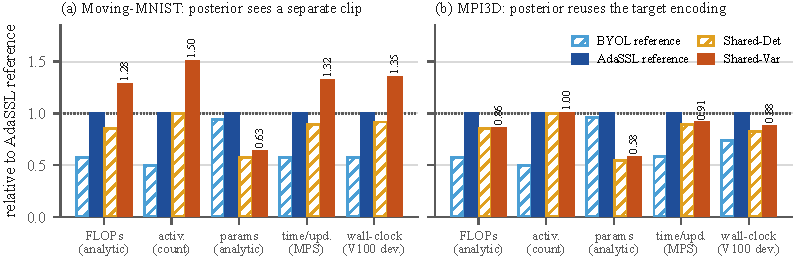
\includegraphics[width=\linewidth]{figures/training_cost.pdf}
\caption{Cost relative to the \emavar{} (post hoc, secondary; lower is better; numbers above bars are \shvar{}'s ratios). FLOPs and parameters are analytic counts, activation memory is a saved-tensor count, time per update is from the controlled benchmark, and wall-clock is from one development run per model. The sign of the \shvar{}$-$\emavar{} difference follows the posterior input.}
\label{fig:cost}
\end{figure}


\begin{table}[htbp]
\caption{Full cost record (post hoc; lower is better in every column; bold marks the lowest value per column and dataset). ``Bench.'' is the benchmark's CPU count of training GFLOPs per update, which appears in Table~\ref{tab:cost}. ``Math attn.'' recounts MPI3D with the math attention backend forced, so that attention matmuls are counted identically in every pass. Under the default backend they are counted in the no-gradient EMA pass but not in gradient-carrying passes; Moving-MNIST has no attention. The recount raises all MPI3D counts by about \VCostMathGain\% and leaves the \shvar{}/\emavar{} ratio unchanged (\VMPCostFlopsRatio{} in both). Saved activations are measured on MPS; the CPU recount with the math backend gives the same values to within 1 MiB. Development wall-clock is in Table~\ref{tab:cost}. ``Sweep 1 / 2'' are the median MPS update times of the two sweeps. Inference MFLOPs are per forecast (number of prior draws or atoms in parentheses), counted with the transformer fast path disabled.}
\label{tab:costfull}
\centering
\small
\setlength{\tabcolsep}{4pt}
\adjustbox{max width=\linewidth}{\begin{tabular}{@{}llrrrrrr@{}}
\toprule
 & & Trainable & \multicolumn{2}{c}{Training GFLOPs} & Saved act. & ms / update & Inference \\
\cmidrule(lr){4-5}
Dataset & Model & params (M) & bench. & math attn. & (MiB) & sweep 1 / 2 & MFLOPs \\
\midrule
Moving-MNIST & \emadet{} & \best{3.674} & \best{134.2} & \best{134.2} & \best{395} & \best{275 / 278} & \best{263} (1) \\
 & \emavar{} & 4.081 & 234.3 & 234.3 & 789 & {478 / 481} & 429 (64) \\
 & \shdet{} & \best{3.674} & 200.6 & 200.6 & 790 & {428 / 428} & \best{263} (1) \\
 & \shvar{} & 4.081 & 300.8 & 300.8 & 1184 & {630 / 632} & 429 (64) \\
\midrule
MPI3D & \emadet{} & \best{5.993} & \best{105.5} & \best{112.0} & \best{394} & \best{58 / 57} & \best{440} (1) \\
 & \emavar{} & 6.399 & 184.4 & 195.6 & 787 & {99 / 99} & 479 (16) \\
 & \shdet{} & \best{5.993} & 157.8 & 167.5 & 788 & {88 / 88} & \best{440} (1) \\
 & \shvar{} & 6.399 & 158.0 & 167.7 & 789 & {90 / 90} & 479 (16) \\
\bottomrule
\end{tabular}
}
\end{table}

\paragraph{Evidence sources.} (1) \emph{Analytic}: parameter counts and training FLOPs per update (forward and backward). Saved-activation memory, the bytes of non-parameter tensors saved for backward, is counted with saved-tensor hooks in the same setting. All three use the final training recipes on synthetic tensors of the real shapes and batch sizes. (2) \emph{Development wall-clock}: the scheduler-reported elapsed time (Slurm \texttt{ElapsedRaw}) of the single development run per model, including start-up, teardown and checkpointing. Moving-MNIST ran on one V100 and MPI3D on four V100s with DDP. (3) \emph{Controlled benchmark}: all eight model--dataset combinations on one Apple-silicon GPU (PyTorch MPS), with 10 warm-up and 100 timed full updates (optimizer, EMA and SIGReg included) per combination, in two sweeps of alternating model order. MPI3D uses its global batch of 64 on the single device, so there is no DDP communication. (4) \emph{Main-run wall-clock}: recorded on the original storage but not retrieved. We make no estimate of it.

\paragraph{Scope and scripts.} Analytic counts cover matmul and convolution operations as seen by \texttt{torch.utils.flop\_counter.FlopCounterMode}. They exclude elementwise, normalization, optimizer, EMA and SIGReg characteristic-function work, and they are not a runtime prediction. Parameter counts agree between the two benchmarks and, on Moving-MNIST, with a capacity count made before training. The MPS benchmark ran PyTorch 2.8.0 on a single Apple-silicon GPU; the main runs used PyTorch 2.5.1 (CUDA 11.8) on V100s. The values come from a benchmarking script, run once on CPU for FLOP counts (one warm-up and two measured updates, inference batch 8) and once on MPS for timing (10 warm-up and 100 timed updates, two sweeps), and from a recount script that forces the math attention backend. Both scripts are part of the codebase. The benchmark's own inference counts for MPI3D are not used. In evaluation mode the transformer fast path is invisible to the counter, so those counts omit the transformer blocks. The recount disables the fast path.

\FloatBarrier
\section{Complete results and Moving-MNIST diagnostics}
\label{app:results}

Tables~\ref{tab:primary-full}--\ref{tab:perrep} and Figures~\ref{fig:physical-full}--\ref{fig:paired} give the complete primary results for both datasets. Figures~\ref{fig:sampling}--\ref{fig:strata} and Tables~\ref{tab:mmcontrols}--\ref{tab:mmresidual} give the Moving-MNIST controls, residual diagnostics, probes and readout fidelity. Appendix~\ref{app:mpi3d-results} gives the MPI3D diagnostics.

\begin{table}[htbp]
\caption{Primary outcome: physical-forecast Energy Score ($\downarrow$ lower is better), as mean $\pm$ sample SD and range over five training replications. Bold marks the lowest mean per dataset, which by itself does not establish superiority (see Table~\ref{tab:paired}). The datasets have different units. Appendix Table~\ref{tab:perrep} lists all 40 values.}
\label{tab:primary-full}
\centering
\small
\begin{tabular}{@{}lcccc@{}}
\toprule
 & \multicolumn{2}{c}{Moving-MNIST ES $\downarrow$ (px/frame)} & \multicolumn{2}{c}{MPI3D ES $\downarrow$ (grid indices)} \\
\cmidrule(lr){2-3}\cmidrule(l){4-5}
Model & mean $\pm$ SD & range & mean $\pm$ SD & range \\
\midrule
\emadet{} & 3.254 $\pm$ 0.245 & 2.866--3.537 & 4.04$\times$10$^{6}$ $\pm$ 4.03$\times$10$^{6}$ & 1.00$\times$10$^{6}$--1.08$\times$10$^{7}$ \\
\emavar{} & 0.777 $\pm$ 0.100 & 0.665--0.881 & 4{,}150 $\pm$ 1{,}881 & 1{,}773--6{,}965 \\
\shdet{} & 1.625 $\pm$ 0.027 & 1.596--1.659 & 7.22 $\pm$ 2.06 & 4.54--9.12 \\
\shvar{} & \best{0.702 $\pm$ 0.124} & 0.641--0.923 & \best{6.35 $\pm$ 2.23} & 4.25--9.40 \\
\bottomrule
\end{tabular}

\end{table}

\begin{table}[htbp]
\caption{Prespecified paired contrasts ($\downarrow$ negative values favour \shvar{}). Intervals are individual paired-$t$ intervals (df $=4$), not simultaneous, and no hypothesis tests were prespecified. ``Runs $<0$'' counts the replications in which \shvar{} scored lower.}
\label{tab:paired}
\centering
\small
\begin{tabular}{@{}llccc@{}}
\toprule
Dataset & Contrast & Mean diff.\ $\downarrow$ & 95\% paired $t$ interval & Runs $<0$ \\
\midrule
Moving-MNIST & \shvar{} $-$ \emavar{} & $-0.075$ & [$-0.320$, $0.170$] & 4 of 5 \\
Moving-MNIST & \shvar{} $-$ \shdet{} & $-0.923$ & [$-1.064$, $-0.782$] & 5 of 5 \\
\midrule
MPI3D & \shvar{} $-$ \emavar{} & $-4{,}144$ & [$-6{,}479$, $-1{,}809$] & 5 of 5 \\
MPI3D & \shvar{} $-$ \shdet{} & $-0.87$ & [$-3.73$, $1.99$] & 2 of 5 \\
\bottomrule
\end{tabular}

\end{table}

\begin{figure}[htbp]
\centering
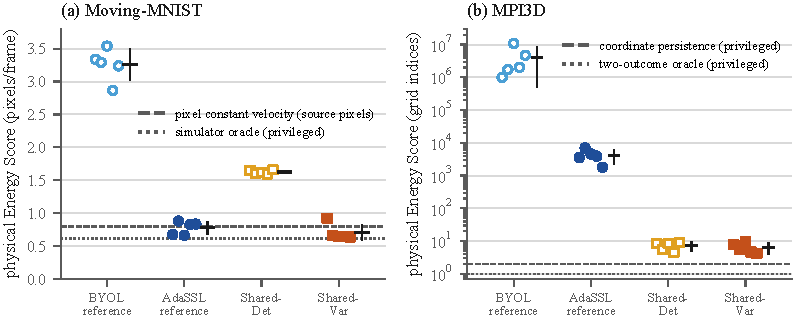
\includegraphics[width=\linewidth]{figures/physical_forecast_results.pdf}
\caption{Physical-forecast Energy Score of all 40 runs (lower is better). Within each model, points are replications 1--5 from left to right. Black marks show the mean $\pm$ sample SD; on the MPI3D log axis the lower end is clipped at half the smallest run. Horizontal lines are shared fixed-bank references: pixel constant velocity uses source pixels only, and the other references are privileged.}
\label{fig:physical-full}
\end{figure}

\begin{table}[htbp]
\caption{All 40 primary outcomes (physical Energy Score, $\downarrow$) and the per-replication paired differences. Bold marks the lowest score in each replication.}
\label{tab:perrep}
\centering
\small
\adjustbox{max width=\linewidth}{\begin{tabular}{@{}llrrrrr@{}}
\toprule
Dataset & Model (ES $\downarrow$) & Rep.~1 & Rep.~2 & Rep.~3 & Rep.~4 & Rep.~5 \\
\midrule
Moving-MNIST & \emadet{} & 3.338 & 3.291 & 3.537 & 2.866 & 3.238 \\
Moving-MNIST & \emavar{} & \best{0.676} & 0.881 & 0.665 & 0.829 & 0.835 \\
Moving-MNIST & \shdet{} & 1.649 & 1.608 & 1.614 & 1.596 & 1.659 \\
Moving-MNIST & \shvar{} & 0.923 & \best{0.656} & \best{0.647} & \best{0.643} & \best{0.641} \\
Moving-MNIST & \shvar{} $-$ \emavar{} & $0.247$ & $-0.224$ & $-0.018$ & $-0.186$ & $-0.194$ \\
Moving-MNIST & \shvar{} $-$ \shdet{} & $-0.726$ & $-0.952$ & $-0.967$ & $-0.953$ & $-1.018$ \\
\midrule
MPI3D & \emadet{} & 1.00$\times$10$^{6}$ & 1.72$\times$10$^{6}$ & 1.08$\times$10$^{7}$ & 2.00$\times$10$^{6}$ & 4.68$\times$10$^{6}$ \\
MPI3D & \emavar{} & 3{,}538 & 6{,}965 & 4{,}550 & 3{,}927 & 1{,}773 \\
MPI3D & \shdet{} & 8.53 & \best{5.48} & \best{8.43} & \best{4.54} & 9.12 \\
MPI3D & \shvar{} & \best{7.93} & 5.58 & 9.40 & 4.60 & \best{4.25} \\
MPI3D & \shvar{} $-$ \emavar{} & $-3{,}530$ & $-6{,}959$ & $-4{,}540$ & $-3{,}922$ & $-1{,}768$ \\
MPI3D & \shvar{} $-$ \shdet{} & $-0.60$ & $0.10$ & $0.97$ & $0.06$ & $-4.86$ \\
\bottomrule
\end{tabular}
}
\end{table}

\begin{figure}[htbp]
\centering
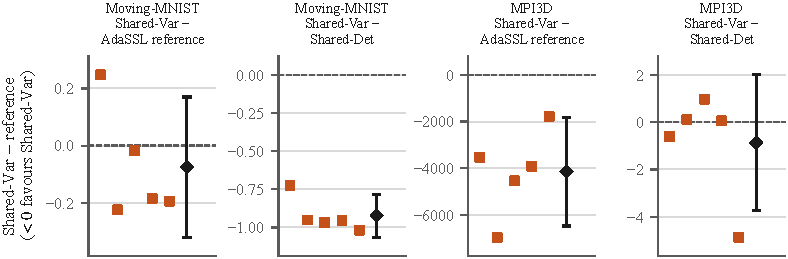
\includegraphics[width=\linewidth]{figures/paired_physical_effects.pdf}
\caption{Primary paired contrasts. Squares are replications 1--5 from left to right; the diamond and bar give the mean and the individual paired-$t$ 95\% interval. Negative values favour \shvar{}. The scales differ by panel.}
\label{fig:paired}
\end{figure}

\begin{figure}[htbp]
\centering
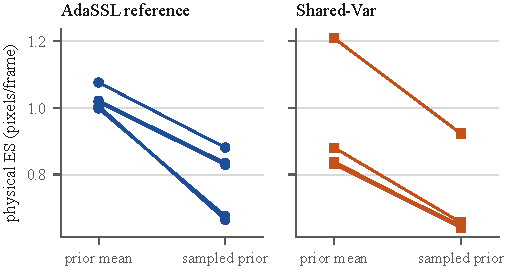
\includegraphics[width=0.68\linewidth]{figures/moving_mnist_sampling_control.pdf}
\caption{Moving-MNIST sampling control. Each of the five lines per panel joins fixed-prior-mean and sampled forecasts from one trained replication. Sampling lowers physical Energy Score in all ten variational-model runs. This inference control retains the trained encoder, predictor and heads.}
\label{fig:sampling}
\end{figure}

\begin{figure}[htbp]
\centering
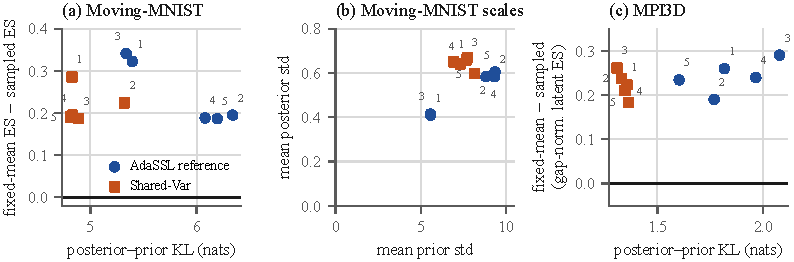
\includegraphics[width=\linewidth]{figures/residual_usage.pdf}
\caption{Residual usage at the end of training, per run; numbers are replication IDs. (a) Moving-MNIST: posterior--prior KL on query trajectories against the gain from sampling over the prior mean. (b) Moving-MNIST: mean prior and posterior standard deviations. (c) MPI3D: posterior--prior KL, averaged over the two outcomes and defined for all 2{,}048 queries, against the sampling gain in the gap-normalized latent score. The posterior is evaluated for diagnosis only and never used to forecast.}
\label{fig:residual}
\end{figure}

\begin{table}[htbp]
\caption{Moving-MNIST forecasts and controls: physical Energy Score, mean $\pm$ SD over five runs (px/frame). Bold marks the lowest mean in the primary row only; controls computed in separately learned target spaces are not ranked.}
\label{tab:mmcontrols}
\centering
\small
\adjustbox{max width=\linewidth}{\begin{tabular}{@{}lcccc@{}}
\toprule
Forecast (physical ES $\downarrow$, px/frame) & \emadet{} & \emavar{} & \shdet{} & \shvar{} \\
\midrule
Sampled prior (primary) & 3.254 $\pm$ 0.245 & 0.777 $\pm$ 0.100 & 1.625 $\pm$ 0.027 & \best{0.702 $\pm$ 0.124} \\
Fixed prior mean & -- & 1.024 $\pm$ 0.031 & -- & 0.918 $\pm$ 0.163 \\
Target-space persistence & 0.836 $\pm$ 0.004 & 0.824 $\pm$ 0.004 & 1.765 $\pm$ 0.119 & 0.863 $\pm$ 0.088 \\
Encode--decode oracle & 0.632 $\pm$ 0.003 & 0.625 $\pm$ 0.002 & 1.278 $\pm$ 0.027 & 0.652 $\pm$ 0.065 \\
Pixel constant velocity & \multicolumn{4}{c}{0.797 (one fixed-bank calculation)} \\
Simulator oracle (privileged) & \multicolumn{4}{c}{0.610 (one fixed-bank calculation)} \\
\bottomrule
\end{tabular}
}
\end{table}

\begin{table}[htbp]
\caption{Moving-MNIST representation probes and readout fidelity (means over five runs). Probes use source clips of the final report bank. The forecast readout is fitted on target-space features of real target clips. The support row gives the mean fraction of predicted features beyond the fit features' 99th-percentile standardized norm. Bold marks the best mean in each row (per axis for $x$/$y$ cells); it does not establish superiority.}
\label{tab:mmrep}
\centering
\small
\adjustbox{max width=\linewidth}{\begin{tabular}{@{}lcccc@{}}
\toprule
Measurement & \emadet{} & \emavar{} & \shdet{} & \shvar{} \\
\midrule
Source backbone, digit accuracy $\uparrow$ & 0.851 & \best{0.891} & 0.878 & 0.843 \\
Source projector, digit accuracy $\uparrow$ & 0.706 & \best{0.852} & 0.621 & 0.517 \\
Source backbone, velocity $R^2$ ($x$ / $y$) $\uparrow$ & 0.974 / 0.969 & 0.984 / 0.985 & 0.986 / 0.986 & \best{0.991} / \best{0.990} \\
Source projector, velocity $R^2$ ($x$ / $y$) $\uparrow$ & 0.988 / 0.987 & \best{0.992} / \best{0.995} & 0.383 / 0.499 & 0.920 / 0.992 \\
Forecast readout, velocity $R^2$ ($x$ / $y$) $\uparrow$ & 0.973 / 0.972 & \best{0.980} / \best{0.976} & 0.146 / 0.163 & 0.904 / \best{0.976} \\
Encode--decode velocity RMSE (px/frame) $\downarrow$ & 0.264 & \best{0.229} & 1.540 & 0.333 \\
Predicted features above fit 99th percentile (fraction) $\downarrow$ & 0.352 & \best{0.000} & 0.117 & 0.016 \\
Selected readout transform  & raw & raw & unit & raw \\
\bottomrule
\end{tabular}
}
\end{table}

\begin{table}[htbp]
\caption{Moving-MNIST residual diagnostics at the end of training (mean $\pm$ SD over five runs). The KL uses posteriors evaluated on query trajectories for diagnosis only. Intervals are empirical 5--95\% marginal intervals from 64 prior draws, evaluated against 128 truth draws. Bold marks the coverage closer to the nominal 0.90.}
\label{tab:mmresidual}
\centering
\small
\begin{tabular}{@{}lcc@{}}
\toprule
Endpoint diagnostic & \emavar{} & \shvar{} \\
\midrule
Posterior--prior KL (nats)  & 5.87 $\pm$ 0.47 & 4.94 $\pm$ 0.22 \\
Mean prior std  & 7.74 $\pm$ 1.99 & 7.58 $\pm$ 0.47 \\
Mean posterior std  & 0.52 $\pm$ 0.10 & 0.64 $\pm$ 0.03 \\
90\% interval coverage, $x$ ($\to$0.90) & 0.679 $\pm$ 0.207 & \best{0.810 $\pm$ 0.169} \\
90\% interval coverage, $y$ ($\to$0.90) & 0.577 $\pm$ 0.104 & \best{0.879 $\pm$ 0.030} \\
90\% interval width, $x$ (px/frame)  & 1.85 $\pm$ 0.89 & 2.19 $\pm$ 0.34 \\
90\% interval width, $y$ (px/frame)  & 1.19 $\pm$ 0.14 & 2.35 $\pm$ 0.28 \\
\bottomrule
\end{tabular}

\end{table}



\begin{figure}[htbp]
\centering
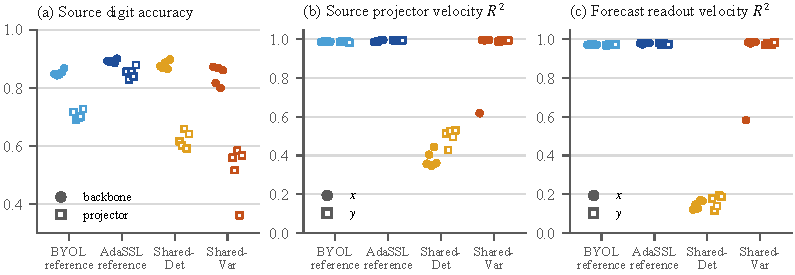
\includegraphics[width=\linewidth]{figures/moving_mnist_representation_tradeoffs.pdf}
\caption{Moving-MNIST representation trade-offs. (a, b) Online source-clip probes. (c) Target-space forecast readout on real target clips. Filled and open markers are the two series named in each legend. Within a series, replications run 1--5 from left to right. \shvar{}'s weak replication 1 is the outlier in (b) and (c); in (a), the low projector digit accuracy (0.361) is replication 4.}
\label{fig:representation}
\end{figure}

\begin{figure}[htbp]
\centering
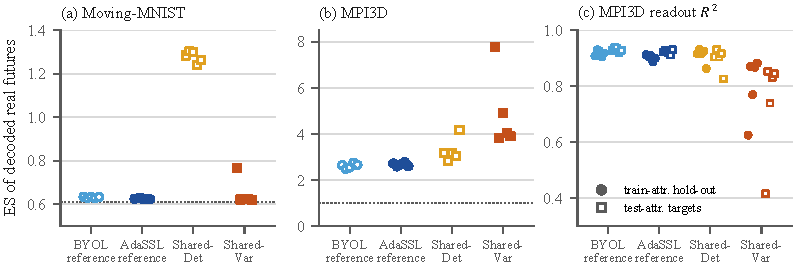
\includegraphics[width=\linewidth]{figures/readout_fidelity.pdf}
\caption{Readout fidelity. (a, b) Energy Score of decoded encodings of real futures (the encode--decode oracle), with the dotted line marking the privileged oracle. (c) MPI3D readout $R^2$ on the in-support training-attribute hold-out (filled) and on real test-attribute targets (open).}
\label{fig:fidelity}
\end{figure}

\begin{figure}[htbp]
\centering
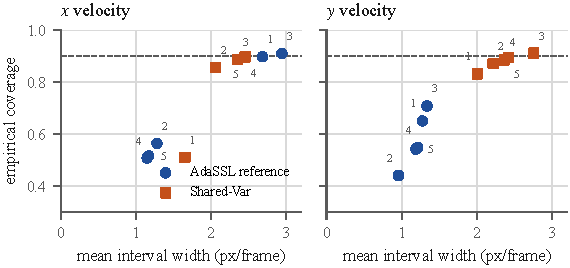
\includegraphics[width=0.72\linewidth]{figures/moving_mnist_interval_coverage.pdf}
\caption{Moving-MNIST empirical 90\% marginal interval coverage against mean width, by axis. Points are runs, labelled by replication ID; the dashed line is the nominal level. Deterministic models have zero width and zero coverage by construction. The estimate depends on the number of draws and is not a calibration proof.}
\label{fig:coverage}
\end{figure}

\begin{figure}[htbp]
\centering
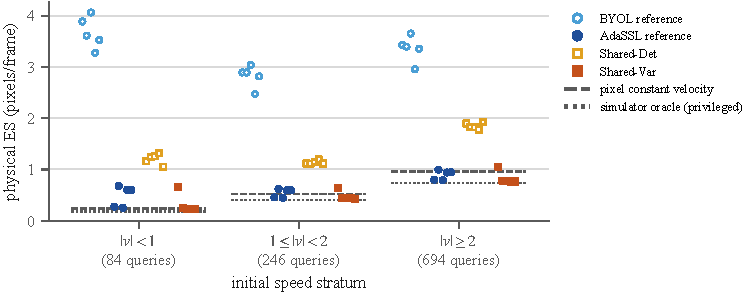
\includegraphics[width=0.9\linewidth]{figures/moving_mnist_speed_strata.pdf}
\caption{Moving-MNIST physical Energy Score by initial-speed stratum (post hoc, secondary). Points are runs. Lines mark the shared pixel constant-velocity baseline and the privileged simulator oracle, each computed once per stratum on the fixed bank.}
\label{fig:strata}
\end{figure}

\FloatBarrier
\section{MPI3D diagnostics: no run beats its latent persistence control}
\label{app:mpi3d-results}

\begin{figure}[htbp]
\centering
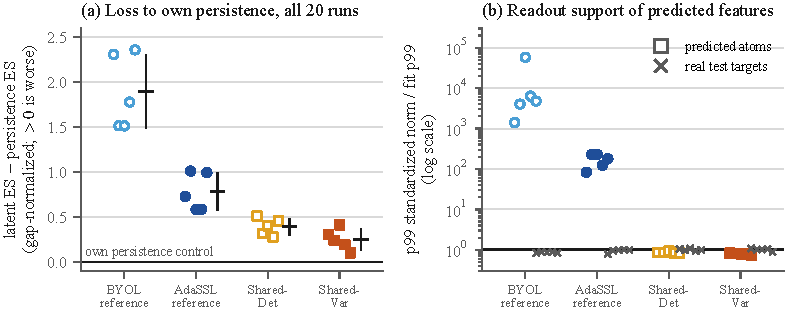
\includegraphics[width=\linewidth]{figures/mpi3d_forecast_failure.pdf}
\caption{MPI3D failure analysis, all 20 runs. (a) Gap-normalized latent Energy Score minus the same model's target-space persistence score (exactly 0.5). Values above zero are worse, and every run is above zero; deterministic models cannot fall below zero by construction. Separately learned spaces admit no cross-model ranking. (b) Ratio of the 99th-percentile standardized norm of predicted atoms (model markers) and of real test-attribute targets ($\times$) to that of the readout's fit features, on a log scale. Every EMA-model predicted atom lies beyond the fit 99th percentile.}
\label{fig:mpi3d}
\end{figure}

\paragraph{Physical scores.} In grid indices, \shvar{} scores \VMPSOneMean{} $\pm$ \VMPSOneSD{} and \shdet{} \VMPSZeroMean{} $\pm$ \VMPSZeroSD. The \emavar{} scores \VMPROneMean{} $\pm$ \VMPROneSD, and the \emadet{} scores \VMPRZeroMean{} $\pm$ \VMPRZeroSD. The \shvar{}$-$\shdet{} difference is $\VMPSOneSZeroDiff$ with interval $[\VMPSOneSZeroLo,\VMPSOneSZeroHi]$, and \shvar{} is lower in only \VMPSOneSZeroWins{} of 5 replications (Figure~\ref{fig:paired}). The interval against the \emavar{} excludes zero. That reflects a numerical failure in the EMA models' pipeline (Figure~\ref{fig:mpi3d}), not a general advantage. Every run of every model is worse than privileged coordinate persistence (2.0).

\paragraph{The EMA models' predictions leave the readout's support.} In every \emadet{} and \emavar{} run, all predicted atoms lie beyond the 99th percentile of the standardized norm of the readout's fit features. Their mean 99th-percentile norms are \VMPRZeroPredNorm{} and \VMPROnePredNorm, against fit percentiles of \VMPFitNormLo--\VMPFitNormHi{} (Figure~\ref{fig:mpi3d}b). Real test targets stay in support. A check made before main training reproduced these extreme outputs in the development runs with independent ridge solves. A plausible but untested explanation is that the cosine loss leaves the scale of the prediction free, while the readout is fitted on raw real features. The Shared models stay in support. The large physical contrasts describe this pipeline failure; on the latent score, neither Shared model beats its own persistence control.

\paragraph{No model beats persistence, independently of the decoder.} In all \VMPLoseToPersistence{} runs, the gap-normalized latent score is worse than the model's own persistence control (Figure~\ref{fig:mpi3d}a). The ten deterministic runs cannot score below it by construction (Appendix~\ref{app:eval}); the ten variational runs could, but none does. \shvar{} averages \VMPSOneLatentES{} (runs: \VMPSOneLatentESList) and \shdet{} \VMPSZeroLatentES, against 0.5 for persistence and 0.25 for the exact distribution. In physical units, \shvar{} beats the decoding of its own persistence (\VMPSOnePhysPersist) in \VMPSOneBeatsOwnPhysPersist{} of 5 runs, but no run approaches privileged coordinate persistence.

\paragraph{Readout transfer and conditioning controls.} On real test-attribute targets, \shvar{}'s readout reaches $R^2=\VMPSOneReadoutTestRtwo$ (replication 1: \VMPSOneReadoutTestRtwoWeak). The other models reach 0.90--0.93. Decoding real outcome images scores \VMPSOneOracleED{} for \shvar{}, against 1.0 for the exact distribution, so the physical scores include substantial readout distortion (Tables~\ref{tab:mpcontrols} and~\ref{tab:mpsupport}). Rotating the command worsens \shvar{}'s latent score in every run (\VMPSOneLatentWrongAction), and a wrong source worsens its physical score to \VMPSOneWrongSource. The forecasts therefore depend on source and command, but this sensitivity does not yield prediction beyond persistence. Online representation probes are in Table~\ref{tab:mpprobes}.

\begin{table}[htbp]
\caption{MPI3D forecasts and controls (means over five runs). The privileged references are single fixed-bank values. Bold marks the lowest mean in the two sampled-prior rows only.}
\label{tab:mpcontrols}
\centering
\small
\adjustbox{max width=\linewidth}{\begin{tabular}{@{}lcccc@{}}
\toprule
Forecast & \emadet{} & \emavar{} & \shdet{} & \shvar{} \\
\midrule
\multicolumn{5}{@{}l}{\emph{Physical Energy Score $\downarrow$ (Euclidean grid indices)}} \\
Sampled prior (primary) & 4.04$\times$10$^{6}$ & 4{,}150 & 7.22 & \best{6.35} \\
Fixed prior mean & -- & 7{,}397 & -- & 7.47 \\
Target-space persistence & 3.80 & 3.91 & 4.29 & 5.92 \\
Wrong command & 4.04$\times$10$^{6}$ & 4{,}150 & 7.95 & 6.79 \\
Wrong source & 4.04$\times$10$^{6}$ & 4{,}150 & 17.64 & 14.36 \\
Encode--decode oracle & 2.61 & 2.67 & 3.26 & 4.88 \\
Coordinate persistence (privileged) & \multicolumn{4}{c}{2.000} \\
Commanded move (privileged) & \multicolumn{4}{c}{2.000} \\
Two-outcome oracle (privileged) & \multicolumn{4}{c}{1.000} \\
\midrule
\multicolumn{5}{@{}l}{\emph{Gap-normalized latent Energy Score $\downarrow$ (within each model's own target space)}} \\
Sampled prior & 2.396 & 1.282 & 0.893 & \best{0.750} \\
Fixed prior mean & -- & 1.525 & -- & 0.974 \\
Target-space persistence & 0.500 & 0.500 & 0.500 & 0.500 \\
Wrong command & 2.403 & 1.328 & 1.061 & 0.920 \\
Wrong source & 2.502 & 1.850 & 9.045 & 8.278 \\
Encode--decode oracle & 0.250 & 0.250 & 0.250 & 0.250 \\
\bottomrule
\end{tabular}
}
\end{table}

\begin{table}[htbp]
\caption{MPI3D readout support and fidelity (means over five runs). Standardized norms use each run's fitted readout and its selected transform. Bold marks the best mean in each directional row; it does not establish superiority.}
\label{tab:mpsupport}
\centering
\small
\adjustbox{max width=\linewidth}{\begin{tabular}{@{}lcccc@{}}
\toprule
Diagnostic & \emadet{} & \emavar{} & \shdet{} & \shvar{} \\
\midrule
Fit features, 99th-percentile standardized norm  & 23.35 & 16.18 & 20.34 & 19.14 \\
Predicted features, 99th-percentile standardized norm  & 3.03$\times$10$^{5}$ & 2{,}662 & 17.59 & 15.12 \\
Real test targets, 99th-percentile standardized norm  & 20.04 & 15.12 & 20.50 & 19.27 \\
Predicted atoms above fit 99th percentile (fraction) $\downarrow$ & 1.0000 & 1.0000 & 0.0004 & \best{0.0000} \\
Real test targets above fit 99th percentile (fraction) $\downarrow$ & \best{0.0015} & 0.0063 & 0.0155 & 0.0132 \\
Readout $R^2$, train-attribute hold-out $\uparrow$ & \best{0.917} & 0.902 & 0.910 & 0.803 \\
Readout $R^2$, real test-attribute targets $\uparrow$ & \best{0.930} & 0.922 & 0.896 & 0.737 \\
Selected readout transform  & raw & raw & raw & raw \\
\bottomrule
\end{tabular}
}
\end{table}

\begin{table}[htbp]
\caption{MPI3D online representation probes on 2{,}048 test-attribute images (means over five runs). Bold marks the highest mean in each row; it does not establish superiority.}
\label{tab:mpprobes}
\centering
\small
\adjustbox{max width=\linewidth}{\begin{tabular}{@{}llcccc@{}}
\toprule
Features & Probe ($\uparrow$) & \emadet{} & \emavar{} & \shdet{} & \shvar{} \\
\midrule
Pooled backbone & Position $R^2$ (mean of axes) & 0.708 & 0.738 & \best{0.899} & 0.878 \\
 & Colour, balanced accuracy & 0.977 & 0.970 & \best{1.000} & 0.999 \\
 & Shape, balanced accuracy & 0.204 & \best{0.220} & 0.074 & 0.061 \\
 & Size, balanced accuracy & 0.824 & 0.826 & \best{0.829} & 0.818 \\
 & Camera height, balanced accuracy & 0.999 & \best{1.000} & \best{1.000} & \best{1.000} \\
\midrule
Projector & Position $R^2$ (mean of axes) & 0.622 & 0.786 & \best{0.897} & 0.774 \\
 & Colour, balanced accuracy & 0.921 & 0.927 & \best{0.997} & \best{0.997} \\
 & Shape, balanced accuracy & 0.192 & \best{0.231} & 0.103 & 0.139 \\
 & Size, balanced accuracy & 0.798 & \best{0.832} & 0.808 & 0.798 \\
 & Camera height, balanced accuracy & 0.997 & 0.998 & \best{1.000} & 0.998 \\
\bottomrule
\end{tabular}
}
\end{table}
